\chapter{Thuyết tương đối hẹp: các hệ quy chiếu, tính đồng thời và phép biến đổi Lorentz}

Thuyết tương đối là nguyên lý cho rằng các định luật vật lý không phụ thuộc vào việc ta dùng hệ quy chiếu quán tính nào để mô tả chúng. Nhiệm vụ đầu tiên của chúng ta là động học: ý nghĩa của không gian, thời gian, chuyển động, sự đồng bộ hóa, và phép biến đổi từ một hệ quy chiếu quán tính sang một hệ khác. Động lực học đến sau, với năng lượng tương đối tính, động lượng, lực, dạng tương tự của phương trình chuyển động Newton, và ý nghĩa của \(E=mc^2\). Một khi cấu trúc đó đã vững chắc, ta có thể tiếp cận thuyết tương đối rộng về mặt khái niệm thông qua không-thời gian cong, chuyển động của các hạt trong một trường hấp dẫn cho trước, các lỗ đen, và sự giãn nở của vũ trụ, mà không cần bắt đầu từ bài toán khó là giải các phương trình trường Einstein.

Cần phân biệt giữa tính chặt chẽ về mặt khái niệm và về mặt toán học. Chúng ta sẽ không dùng một phép gần đúng mà ta biết là sai. Thay vào đó, ta sẽ nhấn mạnh trường hấp dẫn tác động lên đồng hồ, hạt và hình học như thế nào, đồng thời hoãn lại bộ công cụ cần để xây dựng các nghiệm tùy ý của phương trình trường. Thuyết tương đối hẹp phải được trình bày tường minh hơn vì toàn bộ lập luận về sau đều dựa trên động học của nó.

Vì vậy, điểm khởi đầu đúng không phải là một công thức nổi tiếng, mà là một trình bày chính xác về điều mà một người quan sát hiểu là một vị trí và một thời điểm.

\section{Một hệ quy chiếu là một hệ tọa độ vật lý}

Hãy hình dung không gian được lấp đầy bởi một mạng gồm các thước mét mịn đến mức tùy ý. Mỗi nút mạng được gán ba tọa độ không gian, và tại mỗi nút đều có một đồng hồ. Gộp lại, các thước và các đồng hồ ấy tạo thành một hệ quy chiếu.

\begin{definition}
Một \emph{biến cố} là một điều xảy ra tại một vị trí và một thời điểm. Trong một chiều không gian, tọa độ của nó được viết là \((x,t)\); trong ba chiều, chúng là \((x,y,z,t)\).
\end{definition}

Vật lý Newton bổ sung một giả thiết mạnh: mọi đồng hồ lý tưởng đều có thể được đồng bộ hóa một lần là mãi mãi. Thời gian là phổ quát. Một đồng hồ có thể được di chuyển, và một người quan sát có thể mang theo đồng hồ đeo tay, nhưng mọi người đều được giả định là thống nhất về cùng một \(t\) ở mọi nơi. Điều này đôi khi được gọi là thời gian tuyệt đối; ta có thể hình dung nó như thời gian của Thượng đế, một chiếc đồng hồ duy nhất cho toàn thế giới.

Nguyên lý tương đối có trước Einstein. Hình ảnh tự nhiên của nó là một đoàn tàu chuyển động đều đến mức trên đường ray hoàn toàn nhẵn không có gì rung lắc hay xóc nảy. Bên trong tàu, ta có thể tung và bắt các quả bóng đúng như khi ở một đoàn tàu đang đứng tại ga. Trò tung hứng là một thí nghiệm cơ học nhỏ nhưng đầy đủ một cách đáng ngạc nhiên: nó đòi hỏi việc canh thời gian, trọng lực, sự căn chỉnh, và khả năng điều khiển lặp đi lặp lại các quỹ đạo. Nếu tàu chuyển động với vận tốc không đổi, không quy tắc nào trong số đó thay đổi. Một quả bóng ném thẳng lên trên sẽ trở lại đúng bàn tay cũ; đoàn tàu không trượt đi khỏi ngay bên dưới nó. Galileo nhận ra điều này, và Newton diễn đạt nó một cách có hệ thống trong các định luật chuyển động của mình.

Trước Galileo, người ta dễ bị cám dỗ lập luận rằng đoàn tàu đang chạy hẳn phải tiến lên trong lúc quả bóng còn ở trên không, buộc người tung hứng phải với tay ra sau hoặc ra trước để bắt lại nó. Sai lầm là quên rằng quả bóng đã mang sẵn vận tốc ngang của đoàn tàu khi rời tay. Không thí nghiệm nào bị giới hạn trong toa tàu chuyển động êm lại bộc lộ một trạng thái nghỉ tuyệt đối đặc biệt. Chỉ có chuyển động tương đối giữa hai đoàn tàu là quan sát được.

Vì thế, đoàn tàu đứng yên và đoàn tàu chuyển động đều là hai hệ quy chiếu quán tính. Trước Einstein, chúng liên hệ với nhau bằng các phép biến đổi Galileo.

\section{Vẽ không-thời gian}

Tạm thời ta bỏ qua \(y\) và \(z\), vẽ thời gian theo phương thẳng đứng và vị trí \(x\) theo phương ngang. Mỗi điểm trong hình vẽ là một biến cố. Đường \(x=0\) là lịch sử, hay \emph{đường thế giới}, của gốc không gian. Các đường thẳng đứng lân cận \(x=1,2,3,\ldots\) là các đường thế giới của những nút mạng khác. Các đường ngang là tập hợp các biến cố có cùng một thời gian.

\begin{figure}[H]
\centering
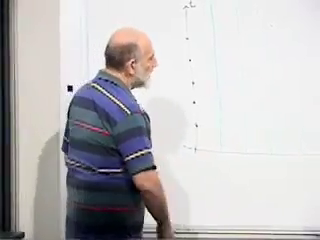
\includegraphics[width=0.62\textwidth]{lecture_01_figure_02.png}
\caption{Trục thời gian của hệ nghỉ và các đường thế giới đầu tiên của mạng không gian.}
\lectureframe{00:16:38}
\end{figure}

Cùng một cách dựng ấy sẽ rõ hơn trong một hình vẽ lý tưởng hóa:

\begin{figure}[H]
\centering
\begin{tikzpicture}[scale=0.95]
\draw[->] (-1.2,0) -- (5.2,0) node[right] {$x$};
\draw[->] (0,-0.2) -- (0,4.8) node[above] {$t$};
\foreach \x in {-1,1,2,3,4}
  \draw[gray!65] (\x,0) -- (\x,4.4);
\foreach \y in {1,2,3,4}
  \draw[gray!65] (-1.0,\y) -- (4.4,\y);
\fill (0,0) circle (1.5pt);
\node[below left] at (0,0) {$0$};
\node[left] at (0,1) {$1$};
\node[left] at (0,2) {$2$};
\node[left] at (0,3) {$3$};
\node[below] at (1,0) {$1$};
\node[below] at (2,0) {$2$};
\node[below] at (3,0) {$3$};
\end{tikzpicture}
\caption{Một mạng không-thời gian đứng yên. Các đường thẳng đứng có vị trí không đổi; các đường ngang có thời gian không đổi.}
\end{figure}

Lưới này là tưởng tượng, và khoảng cách mắt lưới là tùy ý. Ta có thể dùng mét, xentimét, micrômét, hoặc bất kỳ khoảng nhỏ hơn nào nữa mà vẫn có ý nghĩa vật lý. Mục đích của nó là gán một tọa độ chính xác cho mọi biến cố.

Cụm từ “hệ quy chiếu” giờ đây có nội dung thao tác rõ ràng. Nó không chỉ đơn thuần là một góc nhìn hay một người đang nhìn theo hướng nào đó. Nó là một bộ máy tọa độ mở rộng. Với một biến cố cho trước, các thước cục bộ xác định nó xảy ra ở đâu và đồng hồ cục bộ xác định nó xảy ra khi nào. Khi đó ta có thể so sánh các đại lượng vật lý khác giữa các hệ: vị trí và vận tốc của một hạt, năng lượng của nó, có lẽ là nhiệt độ của một vật, và về sau là động lượng và lực của nó. So sánh đơn giản nhất là so sánh liên quan đến \(x\) và \(t\), nên ta bắt đầu từ đó.

Bây giờ đặt một mạng thứ hai trên một đoàn tàu đang chuyển động theo chiều dương của \(x\) với vận tốc không đổi \(v\). Chọn sao cho hai gốc trùng nhau tại \(t=0\). Khi đó gốc chuyển động tuân theo
\begin{equation}
x=vt.
\end{equation}
Mọi điểm khác cố định trên tàu đi theo một đường thế giới nghiêng song song. Độ nghiêng chỉ đơn giản là phát biểu hình học rằng đoàn tàu đổi vị trí khi thời gian trôi qua.

Giả sử điểm phía sau của đoàn tàu là gốc của hệ có phẩy. Tại \(t=0\) nó trùng với gốc của ga. Ở một thời điểm muộn hơn \(t\), tọa độ của nó trong hệ đứng yên là \(vt\). Vì vậy, một biến cố gần đó có tọa độ \(x\) chỉ cách gốc của đoàn tàu một đoạn \(x-vt\). Đây là lý do phép biến đổi là một phép trừ chứ không phải một quy tắc đại số tùy tiện.

Gọi \((x,t)\) là các tọa độ của một biến cố trong hệ của ga và \((x',t')\) là các tọa độ của nó trong hệ của đoàn tàu. Galileo và Newton giữ thời gian phổ quát,
\begin{equation}
t'=t.
\end{equation}
Trong khoảng thời gian \(t\), gốc chuyển động tiến thêm \(vt\), nên khoảng cách từ gốc ấy đến biến cố là
\begin{equation}
x'=x-vt.
\end{equation}
Gộp lại,
\begin{align}
t'&=t, & x'&=x-vt.
\label{eq:galilean-forward}
\end{align}
Giải theo các tọa độ không phẩy cho ta phép biến đổi nghịch,
\begin{align}
t&=t', & x&=x'+vt'.
\label{eq:galilean-inverse}
\end{align}

\begin{figure}[H]
\centering
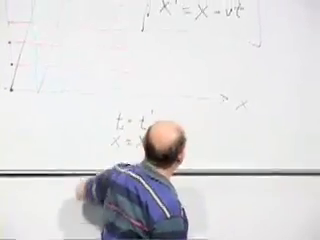
\includegraphics[width=0.72\textwidth]{lecture_01_figure_03.png}
\caption{Phép biến đổi Galileo được viết bên cạnh hai mạng không-thời gian.}
\lectureframe{00:21:57}
\end{figure}

Cặp thứ nhất cho người quan sát chuyển động biết cách chuyển đổi các tọa độ do người quan sát đứng yên cung cấp. Cặp nghịch đảo chuyển đổi theo chiều ngược lại. Sự chuyển đổi hai chiều qua lại giữa các mô tả này là nội dung toán học của thuyết tương đối Galileo.

Việc thay \(t\to t'\) trong công thức không gian nghịch là vô hại chỉ vì lý thuyết Galileo đã tuyên bố sẵn \(t=t'\). Bây giờ lưu ý giả thiết ấy là điều hữu ích. Trong lý thuyết của Einstein, hai tọa độ thời gian sẽ khác nhau, và những phép thay thế như vậy sẽ không còn tự động nữa.

\begin{classroomqa}
\audiencequestion{Nếu mang một đồng hồ đi xa rồi đem trở lại, làm sao ta biết rằng chuyển động của nó không phải là lúc đầu làm nó chạy nhanh hơn rồi sau đó làm nó chạy chậm lại, che lấp hiệu ứng khi so sánh các đồng hồ?
\lecturetimestamp{00:23:09}}
\lecturerresponse{Galileo không thể xác lập thời gian phổ quát với độ chính xác hiện đại; đó là một phỏng đoán vật lý. Ta có thể kiểm tra phỏng đoán ấy bằng nhiều cách: mang các đồng hồ tốt đi theo hai hướng ngược nhau, lặp lại chuyến đi theo hướng bắc--nam cũng như đông--tây, cho một đồng hồ chuyển động vòng quanh chiếc kia, hoặc trao đổi các tín hiệu định thời mà không cần đưa các đồng hồ lại gần nhau. Ở các tốc độ thông thường, mọi phép kiểm tra như vậy đều phù hợp với nhau với độ chính xác rất cao. Với các đồng hồ đủ chính xác hoặc các tốc độ đủ lớn, một sai khác nhỏ quả thật xuất hiện. Việc thời gian phổ quát không còn đúng không phải là khuyết điểm của thí nghiệm; nó là một trong những hiện tượng mà thuyết tương đối hẹp phải giải thích.}
\end{classroomqa}

\section{Các bất biến Galileo và định luật Newton}

Một bất biến là một đại lượng mà mọi người quan sát quán tính đang được xét đều thống nhất. Bản thân các tọa độ không nhất thiết phải bất biến. Điều quan trọng là liệu các định luật được xây dựng từ chúng có giữ nguyên cùng một dạng hay không.

Từ này được dùng vừa như danh từ vừa như tính từ. Một con số có thể là một bất biến, và một phương trình có thể bất biến dưới một phép biến đổi. Sự phân biệt giữa các đại lượng bất biến và các định luật bất biến ngăn ngừa một sự nhầm lẫn thường gặp: thuyết tương đối không khẳng định rằng mọi người quan sát đều thu được cùng một tọa độ cho mọi thứ. Nó khẳng định rằng định luật vật lý nối các phép đo của họ có cùng một dạng.

Xét hai biến cố đồng thời tại các vị trí \(x_1\) và \(x_2\). Phương trình~\eqref{eq:galilean-forward} cho
\begin{align}
x_1'&=x_1-vt,\\
x_2'&=x_2-vt.
\end{align}
Vì thế khoảng cách giữa chúng là
\begin{equation}
x_2'-x_1'=(x_2-vt)-(x_1-vt)=x_2-x_1.
\end{equation}
Trong vật lý Galileo, khoảng cách giữa các biến cố xảy ra cùng một thời gian là bất biến mặc dù từng vị trí riêng lẻ thì không.

\begin{classroomqa}
\audiencequestion{Hai lần xuất hiện của \(t\) trong phép trừ đó có thật sự là cùng một thời gian không?
\lecturetimestamp{00:28:16}}
\lecturerresponse{Có. Ta đã cố ý chọn hai biến cố là \((x_1,t)\) và \((x_2,t)\). Chúng nằm trên cùng một đường ngang thời gian không đổi. Vì vậy hạng chung \(vt\) triệt tiêu. Nếu các biến cố xảy ra ở những thời gian khác nhau, lập luận này sẽ không thiết lập được một khoảng cách không gian bất biến.}
\end{classroomqa}

Bây giờ mô tả một hạt bằng quỹ đạo \(x(t)\). Người quan sát trên tàu gán
\begin{equation}
x'(t)=x(t)-vt.
\end{equation}
Lấy đạo hàm một lần cho quy tắc cộng vận tốc quen thuộc,
\begin{equation}
\frac{dx'}{dt}=\frac{dx}{dt}-v.
\end{equation}
Vị trí và vận tốc phụ thuộc hệ quy chiếu. Một người quan sát chuyển động song song với một mũi tên sẽ thấy nó bay chậm hơn so với người quan sát đứng bên đường ray.

Lấy đạo hàm thêm lần nữa. Vì vận tốc tương đối \(v\) là hằng số,
\begin{equation}
\frac{d^2x'}{dt^2}=\frac{d^2x}{dt^2}.
\end{equation}
Gia tốc là bất biến dưới một phép biến đổi Galileo. Điều này gợi ý mạnh vì sao định luật Newton được viết theo gia tốc chứ không theo vị trí hay vận tốc.

Đây là gia tốc của vật được quan sát, không phải gia tốc của người quan sát trên tàu. Cả hai hệ đều là quán tính, nên không hệ nào gia tốc so với hệ kia. Các vật có thể gia tốc sang trái hoặc sang phải trong bất kỳ mô tả nào, và hai người quan sát đều nhất trí về giá trị của gia tốc ấy mặc dù họ bất đồng về vị trí và vận tốc của vật.

Giả sử hai hạt tác dụng lực lên nhau và lực chỉ phụ thuộc vào khoảng cách đồng thời giữa chúng. Khoảng cách ấy là bất biến, nên lực là bất biến. Nếu khối lượng cũng là một tính chất nội tại, độc lập với hệ quy chiếu, thì mọi người quan sát quán tính đều có thể viết
\begin{equation}
F=ma
\end{equation}
ở đúng cùng một dạng. Cơ học Newton là bất biến dưới các phép biến đổi Galileo. Điều đó không chỉ là điều có vẻ hợp lý; trong toàn bộ miền tốc độ thông thường, nó cực kỳ chính xác.

Lập luận này áp dụng cho các lực trung tâm quen thuộc như hấp dẫn Newton hay tĩnh điện học, trong đó độ lớn là một hàm của khoảng cách. Vì mọi người quan sát trong cơ học Galileo đều thống nhất về khoảng cách ấy tại cùng một thời gian, họ thống nhất về lực. Khi lực và gia tốc đã cố định, tính nhất quán khi đó buộc họ cũng phải thống nhất về khối lượng: một vật một kilôgam vẫn là một vật một kilôgam khi được chở ngang qua trên một đoàn tàu. Mọi ký hiệu trong \(F=ma\) đều phù hợp với cùng một cấu trúc bất biến.

\section{Ánh sáng không phù hợp với quy tắc Galileo}

Điện từ học gây ra khó khăn. Các phương trình Maxwell dự đoán những sóng truyền qua không gian rỗng với tốc độ xác định \(c\). Nếu các phương trình Maxwell là các định luật tự nhiên và các định luật tự nhiên là như nhau trong mọi hệ quy chiếu quán tính, thì mọi người quan sát quán tính đều phải thu được cùng một \(c\).

Động học Galileo lại dự đoán điều khác. Một xung ánh sáng truyền sang phải trong hệ đứng yên thỏa mãn
\begin{equation}
x=ct.
\end{equation}
Áp dụng phép biến đổi không gian cho ta
\begin{equation}
x'=x-vt=(c-v)t.
\end{equation}
Vì \(t'=t\), người quan sát trên tàu sẽ đo được tốc độ \(c-v\).

Mâu thuẫn có thể được phát biểu dứt khoát. Nếu các phương trình Maxwell giữ nguyên dạng của chúng, chúng dự đoán \(c\) trong hệ có phẩy. Nếu vẫn giữ phép biến đổi Galileo, nó dự đoán \(c-v\). Không thể cả hai đều đúng một cách chính xác khi \(v\ne0\).

Kết quả này trông hoàn toàn tự nhiên nếu ánh sáng ứng xử như một sóng thông thường trong một môi trường. Một chiếc thuyền chuyển động cùng với sóng nước sẽ đo được tốc độ tương đối của sóng thấp hơn. Một người nghe chuyển động trong không khí đứng yên sẽ đo được một tốc độ âm thanh bị dịch đi bởi chuyển động của người đó so với không khí. Vì thế, các nhà vật lý thế kỷ 19 đã đi đến một trạng thái đứng yên ưu tiên, một hệ quy chiếu ête trong đó các phương trình Maxwell có dạng đơn giản nhất và ánh sáng truyền với tốc độ \(c\). Các thí nghiệm được thiết kế để phát hiện chuyển động tương đối so với một hệ quy chiếu ưu tiên như vậy đã không tìm thấy hiệu ứng tương ứng nào.

Có một số cách bố trí thí nghiệm khả dĩ, nhưng mục tiêu chung của chúng là so sánh sự truyền ánh sáng đối với các quan sát viên ở những trạng thái hoặc phương chuyển động khác nhau. Không thí nghiệm nào cho thấy độ dịch Galile như mong đợi. Sự thất bại đó không phải là một phiền toái kỹ thuật nhỏ nhặt. Nó buộc người ta phải lựa chọn giữa nguyên lý tương đối, các phương trình Maxwell và những quan niệm được thừa hưởng về không gian và thời gian.

Einstein tiếp cận xung đột này một cách trực diện hơn. Khi còn trẻ, ông hình dung mình đuổi theo một sóng ánh sáng. Nếu ông có thể bắt kịp nó, mẫu điện từ dao động của nó sẽ đứng yên đông cứng trong không gian, thế nhưng các phương trình Maxwell không cho phép một sóng ánh sáng đứng yên như vậy. Ông chọn xem lý thuyết Maxwell và nguyên lý tương đối là nền tảng, rồi xem xét lại những giả thiết ẩn trong các tọa độ của chúng ta.

Sự xây dựng lại này dựa trên hai tiên đề:
\begin{enumerate}
\item Các định luật vật lý có cùng dạng trong mọi hệ quy chiếu quán tính.
\item Ánh sáng trong chân không có cùng tốc độ \(c\) trong mọi hệ quy chiếu quán tính.
\end{enumerate}

Tiên đề thứ hai không thể cùng tồn tại với phép biến đổi Galile. Phải thay đổi một điều gì đó sâu hơn quy tắc cộng vận tốc. Lựa chọn tối giản của Einstein là giữ lại hai tiên đề ấy và xem xét lại phương trình Galile tưởng như vô hại \(t'=t\).

\section{Đồng bộ hóa các đồng hồ ở xa}

Các khoảng cách trong không gian có thể được xác lập bằng các thanh đo, nhưng các đồng hồ ở xa đòi hỏi một quy ước đồng bộ hóa. Đặt hai đồng hồ ở những khoảng cách bằng nhau đối với một quan sát viên ở trung điểm. Khi mỗi đồng hồ ở đầu mút chỉ đúng thời điểm đã định, hãy để nó phát ra một chớp sáng. Nếu hai chớp sáng đến trung điểm cùng lúc, hãy gọi hai đồng hồ ở đầu mút là đã đồng bộ. Nếu một chớp đến trước, hãy điều chỉnh đồng hồ tương ứng rồi lặp lại quy trình.

Từ \emph{trung điểm} được định nghĩa bằng các thanh đo đã được đặt ra trong chính hệ đó. Vì vậy, phép kiểm tra này chứa hai thành phần tách biệt: khoảng cách không gian bằng nhau tới hai đầu mút và thời điểm đến bằng nhau của các tín hiệu. Không thể bỏ đi thành phần nào. Lặp lại quy trình ấy trên toàn bộ mạng lưới sẽ cho các đường ngang thời gian không đổi mà Newton chỉ đơn giản giả định sẵn.

Định nghĩa này dùng ánh sáng vì tiên đề gán cho ánh sáng cùng một tốc độ trong mọi hệ quy chiếu quán tính. Khi mọi cặp lân cận đều đã được xử lý theo cách này, toàn bộ mạng lưới sẽ mang một hệ đồng hồ đồng bộ.

Bây giờ hãy để một mạng lưới thứ hai chuyển động qua mạng thứ nhất. Trung điểm của thiết bị chuyển động vẫn nằm đúng giữa hai đầu mút đang chuyển động của nó trong chính hệ của nó. Tuy nhiên, so với thiết bị đứng yên, nó chuyển động về phía một chớp tới và rời xa chớp kia. Những chớp được phát ra đồng thời theo các đồng hồ đứng yên không đến cùng lúc tại trung điểm đang chuyển động. Vì quan sát viên chuyển động áp dụng cùng quy tắc trung điểm-và-ánh sáng, nên người đó không thể gọi những lần phát ấy là đồng thời. Mỗi hệ tự đồng bộ hóa các đồng hồ của mình một cách nhất quán, nhưng hai cách đồng bộ đó bất đồng với nhau.

Đây không phải là một ảo giác quang học do thời gian truyền hữu hạn của ánh sáng gây ra. Mỗi quan sát viên đều biết rằng ánh sáng cần thời gian để tới nơi và hiệu chỉnh điều đó bằng cùng tốc độ \(c\). Sự bất đồng vẫn còn sau hiệu chỉnh ấy vì các quan sát viên không chọn cùng một cặp sự kiện ở xa làm một cặp đồng thời. Chính tính đồng thời, chứ không chỉ vẻ bề ngoài của tính đồng thời, là tương đối.

\begin{classroomqa}
\audiencequestion{Liệu ta có thể tránh kết luận này bằng cách đồng bộ hóa đồng hồ bằng âm thanh thay vì bằng ánh sáng không?
\lecturetimestamp{00:49:03}}
\lecturerresponse{Âm thanh dùng được như một tín hiệu đồng bộ hóa trong một hệ quy chiếu mà không khí đứng yên, nhưng tốc độ đo được của nó không như nhau trong mọi hệ quy chiếu quán tính. Một đoàn tàu hở chuyển động trong không khí đứng yên thì chuyển động tương đối so với môi trường truyền âm, nên các tín hiệu âm thanh về phía trước và về phía sau không ứng xử đối xứng ở đó. Theo tiên đề, ánh sáng thì khác: không có môi trường quang học nào có thể phát hiện được mà hệ nghỉ của nó chọn ra một quan sát viên nào đó. Vì vậy, ta dùng ánh sáng và theo các hệ quả của việc đó.}
\end{classroomqa}

Sự bất đồng về mặt định tính đã rõ. Bây giờ ta tính chính xác những sự kiện nào được quan sát viên chuyển động gọi là đồng thời.

\section{Phép dựng bằng tia sáng}

Đối với phép dựng này, thuận tiện nhất là chọn các đơn vị sao cho
\begin{equation}
c=1.
\end{equation}
Khi đó, một đơn vị khoảng cách chính là quãng đường ánh sáng đi được trong một đơn vị thời gian: giây ánh sáng đi cùng với giây, hoặc năm ánh sáng đi cùng với năm. Không gian và thời gian mang cùng đơn vị, các vận tốc là vô thứ nguyên, và các tia sáng hiện ra ở góc \(45^\circ\). Một tia chuyển động sang phải có
\begin{equation}
x=t+d,
\end{equation}
trong khi một tia chuyển động sang trái có
\begin{equation}
x=-t+d'.
\end{equation}
Hai tia đi qua gốc tọa độ đơn giản là \(x=t\) và \(x=-t\). Các đường thế giới kiểu thời gian, thuộc về các vật chậm hơn ánh sáng, nằm gần trục thẳng đứng hơn. Một đường thế giới siêu quang giả định sẽ nằm gần trục ngang hơn.

Góc trong hình vẽ chỉ có ý nghĩa sau khi chọn đơn vị như vậy. Nếu dùng mét và giây, một tia sáng sẽ trông gần như nằm ngang vì nó đi được xấp xỉ \(3\times10^8\) mét trong một giây. Việc chọn giây ánh sáng cho khoảng cách sẽ đổi lại tỷ lệ của trục ngang và làm cho hình học nhân quả trở nên nhìn thấy được.

Xét ba đường thế giới song song trong mạng lưới chuyển động,
\begin{equation}
x=vt,\qquad x=vt+L,\qquad x=vt+2L.
\label{eq:moving-worldlines}
\end{equation}
Đường thế giới ở giữa thuộc về quan sát viên kiểm tra tính đồng thời giữa hai điểm ngoài cùng. Cả ba điểm đều chuyển động đều và giữ nguyên sự sắp xếp tương đối của chúng trong hệ có dấu phẩy.

\begin{figure}[H]
\centering
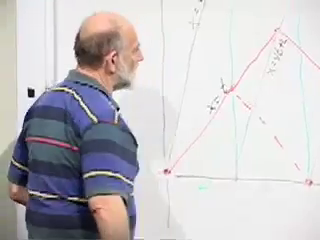
\includegraphics[width=0.72\textwidth]{lecture_01_figure_04.png}
\caption{Tia sáng truyền sang phải \(x=t\) cắt đường thế giới chuyển động ở giữa.}
\lectureframe{01:02:33}
\end{figure}

Có thể vẽ toàn bộ hình học mà không bị một người đứng trước bảng che khuất:

\begin{figure}[H]
\centering
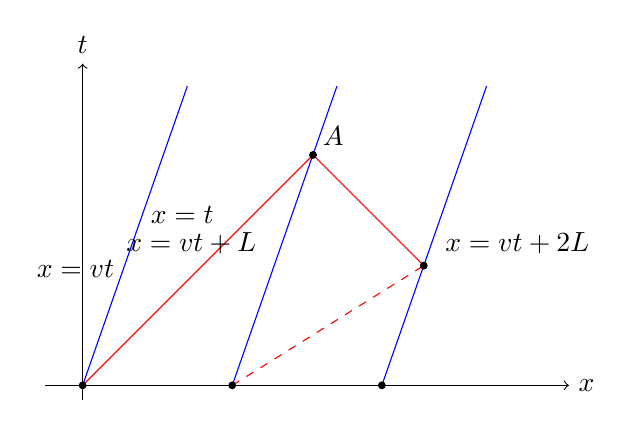
\begin{tikzpicture}[scale=0.95]
\draw[->] (-0.5,0) -- (6.5,0) node[right] {$x$};
\draw[->] (0,-0.2) -- (0,4.3) node[above] {$t$};
\draw[blue] (0,0) -- (1.4,4.0);
\draw[blue] (2.0,0) -- (3.4,4.0);
\draw[blue] (4.0,0) -- (5.4,4.0);
\draw[red] (0,0) -- (3.08,3.08);
\draw[red] (3.08,3.08) -- (4.56,1.60);
\draw[red,dashed] (2.0,0) -- (4.56,1.60);
\fill (0,0) circle (1.5pt);
\fill (2.0,0) circle (1.5pt);
\fill (4.0,0) circle (1.5pt);
\fill (3.08,3.08) circle (1.5pt);
\fill (4.56,1.60) circle (1.5pt);
\node[left] at (0.55,1.55) {$x=vt$};
\node[left] at (2.45,1.9) {$x=vt+L$};
\node[right] at (4.72,1.9) {$x=vt+2L$};
\node[left] at (1.88,2.28) {$x=t$};
\node[above right] at (3.08,3.08) {$A$};
\end{tikzpicture}
\caption{Các tín hiệu ánh sáng xác định đường đồng thời của hệ quy chiếu chuyển động.}
\end{figure}

Cho một tia sáng truyền sang phải xuất phát từ gốc tọa độ. Gọi \(A\) là giao điểm của nó với đường thế giới ở giữa. Hai phương trình tại \(A\) là
\begin{align}
x&=t,\\
x&=vt+L.
\end{align}
Thế vào ta được
\begin{equation}
t=vt+L,
\end{equation}
và do đó
\begin{equation}
t_A=x_A=\frac{L}{1-v}.
\label{eq:point-a}
\end{equation}

Từ \(A\), lần ngược một tia sáng truyền sang trái tới đường thế giới chuyển động ngoài cùng bên phải. Phương trình của nó có dạng
\begin{equation}
x+t=b.
\end{equation}
Vì nó đi qua \(A\), Phương trình~\eqref{eq:point-a} xác định hằng số:
\begin{equation}
b=x_A+t_A=\frac{2L}{1-v}.
\end{equation}
Vì vậy tia đi ngược thỏa mãn
\begin{equation}
x+t=\frac{2L}{1-v}.
\label{eq:backward-ray}
\end{equation}

Giao điểm của nó với đường thế giới ngoài cùng bên phải được suy ra từ
\begin{align}
x+t&=\frac{2L}{1-v},\\
x&=vt+2L.
\end{align}
Loại \(x\) đi,
\begin{align}
(1+v)t
  &=2L\left(\frac{1}{1-v}-1\right)\\
  &=\frac{2Lv}{1-v},
\end{align}
nên
\begin{equation}
t=\frac{2Lv}{1-v^2}.
\end{equation}
Thế vào \(x=vt+2L\) cho
\begin{equation}
x=\frac{2L}{1-v^2}.
\end{equation}
Bản thân các tọa độ kém quan trọng hơn tỷ số của chúng:
\begin{equation}
\frac{t}{x}=v.
\end{equation}
Vì vậy mọi sự kiện đồng thời với gốc tọa độ theo các đồng hồ chuyển động đều nằm trên
\begin{equation}
t=vx,
\label{eq:simultaneity-c-one}
\end{equation}
trong khi gốc tọa độ chuyển động đi theo
\begin{equation}
x=vt.
\label{eq:moving-time-axis}
\end{equation}
Hai trục nghiêng đối xứng quanh tia sáng \(45^\circ\).

Mọi điểm trên \(x=vt\) đều có cùng vị trí có dấu phẩy, \(x'=0\), trong khi thời gian có dấu phẩy của chúng biến thiên. Mọi điểm trên \(t=vx\) đều có cùng thời gian có dấu phẩy, \(t'=0\), trong khi vị trí có dấu phẩy của chúng biến thiên. Vì thế một đường là trục thời gian có dấu phẩy và đường kia là trục không gian có dấu phẩy. Cần đến phép dựng tín hiệu dài dòng ấy để xác định đường thứ hai; không thể suy ra nó chỉ từ riêng đường thế giới chuyển động.

Khôi phục các đơn vị thông thường trong Phương trình~\eqref{eq:simultaneity-c-one} đòi hỏi
\begin{equation}
t=\frac{v}{c^2}x.
\label{eq:simultaneity-dimensional}
\end{equation}
Thừa số \(c^2\) giải thích vì sao bức tranh Newton hoạt động tốt đến vậy trong đời sống hằng ngày. Với các vận tốc rất nhỏ so với \(c\), độ dốc của đường đồng thời chuyển động là cực kỳ nhỏ.

\begin{figure}[H]
\centering
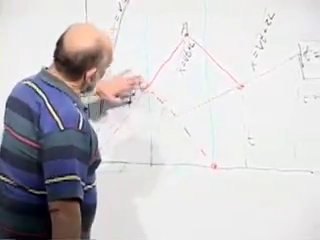
\includegraphics[width=0.72\textwidth]{lecture_01_figure_05.png}
\caption{Với \(c=1\), trục thời gian có dấu phẩy và trục đồng thời đối xứng nhau qua tia sáng.}
\lectureframe{01:15:40}
\end{figure}

\begin{figure}[H]
\centering
\begin{tikzpicture}[scale=1.0]
\draw[->] (-2.2,0) -- (5.2,0) node[right] {$x$};
\draw[->] (0,-0.2) -- (0,4.9) node[above] {$t$};
\draw[red] (0,0) -- (3.9,3.9);
\draw[red] (0,0) -- (-1.8,1.8);
\draw[blue] (0,0) -- (1.8,4.5);
\draw[blue,dashed] (0,0) -- (4.5,1.8);
\node[right] at (3.9,3.9) {$x=t$};
\node[left] at (-1.8,1.8) {$x=-t$};
\node[above] at (1.8,4.5) {$x'=0$};
\node[right] at (4.5,1.8) {$t'=0$};
\end{tikzpicture}
\caption{Các trục có dấu phẩy và các tia sáng bất biến khi dùng các đơn vị \(c=1\).}
\end{figure}

\section{Suy ra phép biến đổi Lorentz}

Hình học xác định nơi mỗi tọa độ có dấu phẩy triệt tiêu. Dọc theo trục thời gian chuyển động \(x=vt\), ta phải có \(x'=0\). Dọc theo trục đồng thời chuyển động \(t=vx\), ta phải có \(t'=0\). Các quan hệ tuyến tính tổng quát nhất có đúng những tập triệt tiêu đó có thể viết thành
\begin{align}
x'&=\frac{x-vt}{F(v)},\\
t'&=\frac{t-vx}{G(v)}.
\label{eq:fg-ansatz}
\end{align}
Các thừa số \(F\) và \(G\) cho phép thang đo của các tọa độ có dấu phẩy khác với các thang đo Galile dù các trục đã được xác định. Tính tuyến tính suy ra từ tính đồng nhất của không gian và thời gian: tịnh tiến một thí nghiệm không thể làm thay đổi quy luật biến đổi.\editorialnote{Lập luận ngắn gọn này về tính tuyến tính làm tường minh một giả thiết đã được dùng ngầm trong phép suy diễn trên bảng.}

Ở giai đoạn này, hình học đã cho ta biết rất nhiều nhưng chưa phải mọi thứ. Các tử số xác định độ nghiêng của các trục. Chúng không xác định khoảng cách đơn vị dọc theo các trục ấy. Chính phần thông tin về thang đo còn lại đó là điều mà \(F(v)\) và \(G(v)\) biểu diễn.

Bây giờ áp đặt tính bất biến của tốc độ ánh sáng. Một tia truyền sang phải thỏa \(x=t\) cũng phải thỏa \(x'=t'\). Dọc theo tia ấy,
\begin{align}
x'&=\frac{(1-v)t}{F(v)},\\
t'&=\frac{(1-v)t}{G(v)}.
\end{align}
Đẳng thức tại mọi điểm trên tia đòi hỏi
\begin{equation}
F(v)=G(v).
\end{equation}
Vì vậy ta có thể viết
\begin{align}
x'&=\frac{x-vt}{F(v)},\\
t'&=\frac{t-vx}{F(v)}.
\label{eq:common-f}
\end{align}

Bước này sử dụng đòi hỏi đầu tiên thật sự mang tính Einstein trong phần đại số. Cùng một đường hình học là một tia sáng đối với cả hai quan sát viên, nên hai tọa độ có dấu phẩy phải tăng như nhau dọc theo nó khi \(c=1\). Những thừa số khác nhau trong hai phương trình sẽ làm cho tốc độ có dấu phẩy khác 1.

Còn lại một hàm chưa biết. Nhân Phương trình~\eqref{eq:common-f} với \(F(v)\):
\begin{align}
F(v)x'&=x-vt,\\
F(v)t'&=t-vx.
\end{align}
Nhân phương trình thứ hai với \(v\) rồi cộng vào phương trình thứ nhất sẽ khử \(t\), ta được
\begin{equation}
(1-v^2)x=F(v)(x'+vt').
\end{equation}
Tương tự,
\begin{equation}
(1-v^2)t=F(v)(t'+vx').
\end{equation}
Vì thế phép biến đổi nghịch đảo là
\begin{align}
x&=\frac{F(v)}{1-v^2}(x'+vt'),\\
t&=\frac{F(v)}{1-v^2}(t'+vx').
\end{align}

Nguyên lý tương đối khiến hai hệ quy chiếu là tương hỗ. Nếu nhà ga thấy đoàn tàu chuyển động với \(+v\), thì đoàn tàu thấy nhà ga chuyển động với \(-v\). Do đó các phương trình nghịch đảo phải có cùng dạng với các phương trình thuận khi đổi dấu \(v\). Các hệ số đứng trước của chúng phải thỏa
\begin{equation}
\frac{F(v)}{1-v^2}=\frac{1}{F(v)}.
\end{equation}
Suy ra
\begin{equation}
F(v)^2=1-v^2,
\end{equation}
và tính liên tục với phép biến đổi đồng nhất tại \(v=0\) chọn nghiệm dương,
\begin{equation}
F(v)=\sqrt{1-v^2}.
\end{equation}

Không có gì ở đây được điều chỉnh để khớp với một xung ánh sáng cụ thể nào. Kết quả suy ra từ các trục được cố định bởi phép đồng bộ hóa, từ tốc độ chung của ánh sáng và từ yêu cầu rằng không hệ quy chiếu quán tính nào được ưu tiên hơn hệ kia.

Phép biến đổi Lorentz trong các đơn vị với \(c=1\) là
\begin{align}
x'&=\frac{x-vt}{\sqrt{1-v^2}},\\
t'&=\frac{t-vx}{\sqrt{1-v^2}}.
\label{eq:lorentz-c-one}
\end{align}
Nghịch đảo của nó là
\begin{align}
x&=\frac{x'+vt'}{\sqrt{1-v^2}},\\
t&=\frac{t'+vx'}{\sqrt{1-v^2}}.
\end{align}

\begin{figure}[H]
\centering
\includegraphics[width=0.76\textwidth]{lecture_01_figure_06.png}
\caption{Phép biến đổi Lorentz với \(c=1\) ở dạng hoàn chỉnh trên bảng.}
\lectureframe{01:32:38}
\end{figure}

Điểm mới cốt yếu đã hiện rõ ngay trong phương trình thời gian. Thời gian không đơn giản được chuyển nguyên vẹn từ hệ này sang hệ kia. Một tọa độ thời gian có dấu phẩy pha trộn thời gian và vị trí không dấu phẩy. Hệ quả là \(t=\text{constant}\) và \(t'=\text{constant}\) mô tả những tập sự kiện khác nhau.

Hạng trộn này không phải là một hiệu chỉnh tùy chọn được gắn thêm về sau. Không có nó, đường \(t'=0\) sẽ vẫn nằm ngang, tính đồng thời ở xa sẽ vẫn là phổ quát, và phép biến đổi sẽ không thể bảo toàn tốc độ ánh sáng.

\section{Khôi phục tốc độ ánh sáng và kiểm tra kết quả}

Khi \(c\ne1\), tính nhất quán thứ nguyên khôi phục các thừa số còn thiếu. Tỉ số \(v^2/c^2\) là vô thứ nguyên, còn \((v/c^2)x\) có đơn vị thời gian. Vì thế
\begin{align}
x'&=\frac{x-vt}{\sqrt{1-v^2/c^2}},\\
t'&=\frac{t-(v/c^2)x}{\sqrt{1-v^2/c^2}}.
\label{eq:lorentz-dimensional}
\end{align}
Nghịch đảo thu được bằng cách đổi dấu \(v\):
\begin{align}
x&=\frac{x'+vt'}{\sqrt{1-v^2/c^2}},\\
t&=\frac{t'+(v/c^2)x'}{\sqrt{1-v^2/c^2}}.
\end{align}
Việc đưa vào
\begin{equation}
\gamma=\frac{1}{\sqrt{1-v^2/c^2}}
\end{equation}
sẽ đưa chúng về dạng gọn quen thuộc, nhưng dạng viết qua mẫu số này giữ cho phép suy diễn vẫn hiện rõ.

Về mặt số trị, \(c\simeq3\times10^8\,\mathrm{m/s}\), nên \(c^2\simeq9\times10^{16}\,\mathrm{m^2/s^2}\). Mẫu số lớn làm cho cả độ nghiêng của đường đồng thời lẫn thừa số \(v^2/c^2\) đều không thể nhận thấy trong phần lớn các thí nghiệm cơ học. Sự nhỏ bé của chúng giải thích thành công của Galileo; nó không khôi phục thời gian tuyệt đối.

\begin{figure}[H]
\centering
\includegraphics[width=0.76\textwidth]{lecture_01_figure_07.png}
\caption{Phép biến đổi Lorentz sau khi đã khôi phục các thừa số \(c\).}
\lectureframe{01:35:58}
\end{figure}

Có thể kiểm tra ngay hai điều. Trước hết, xét \(v\ll c\). Khi đó \(v^2/c^2\) là không đáng kể, và với các khoảng cách thông thường thì số hạng \(vx/c^2\) biểu thị tính tương đối của sự đồng thời cũng không đáng kể. Phương trình~\eqref{eq:lorentz-dimensional} rút gọn thành
\begin{equation}
t'\approx t,\qquad x'\approx x-vt.
\end{equation}
Phép tương đối Galileo được khôi phục như gần đúng tốc độ thấp.

Thứ hai, hãy kiểm tra một tia sáng. Sau khi \(c\) đã được khôi phục, một tia truyền sang phải thỏa mãn \(x=ct\), không phải \(x=t\). Thế vào, ta được
\begin{align}
x'&=\frac{(c-v)t}{\sqrt{1-v^2/c^2}},\\
t'&=\frac{(1-v/c)t}{\sqrt{1-v^2/c^2}}.
\end{align}
Vì \(c-v=c(1-v/c)\),
\begin{equation}
x'=ct'.
\end{equation}
Người quan sát ở hệ phẩy đo được cùng tốc độ \(c\). Với một tia truyền sang trái, việc thay \(x=-ct\) vào tương tự cho
\begin{equation}
x'=-ct'.
\end{equation}
Phép biến đổi xử lý đúng ánh sáng truyền theo cả hai hướng.

Sự phân biệt giữa \(x=t\) và \(x=ct\) là một phép kiểm tra thứ nguyên rất bổ ích. Biểu thức thứ nhất chỉ đúng trong hệ đơn vị mà \(c=1\). Việc khôi phục các đơn vị thông thường trong phép biến đổi mà vẫn để phương trình tia ở đơn vị tự nhiên sẽ trộn lẫn hai quy ước và cho ra một kết quả sai. Tính nhất quán thứ nguyên phát hiện sai lầm đó ngay lập tức.

\section{Tiêu chuẩn trung điểm}

\begin{classroomqa}
\audiencequestion{Giả sử một người quan sát nhận được hai chớp sáng vào cùng một thời điểm nhưng không ở chính giữa hai nguồn phát của chúng. Người quan sát đó có thể kết luận rằng hai chớp sáng đã được phát ra đồng thời không?
\lecturetimestamp{01:42:55}}
\lecturerresponse{Không. Thời điểm đến bằng nhau chỉ kéo theo thời điểm phát bằng nhau đối với người quan sát nằm đúng tại trung điểm không gian giữa hai nguồn trong hệ quy chiếu thích hợp. Một máy thu ở gần một nguồn hơn vẫn có thể nhận đồng thời cả hai chớp sáng, mặc dù chớp sáng ở xa hơn đã được phát ra sớm hơn. Vì vậy, trong dựng hình chuyển động, đường thế giới trung điểm \(x=vt+L\) là thiết yếu. Tia đi sang phải \(x=t\) được theo dõi cho đến khi gặp trung điểm đó, rồi một tia sáng ngược chiều được lần theo tới \(x=vt+2L\). Biến cố đầu mút thứ hai ấy, chứ không phải một biến cố nhận đồng thời tùy ý ở nơi khác, mới đồng thời với gốc theo hệ quy chiếu chuyển động.}
\end{classroomqa}

Chúng ta đã đi tới phép biến đổi tọa độ đầy đủ, nhưng chưa tới những hệ quả quen thuộc nhất của nó. Tiếp theo sẽ là sự co độ dài, sự giãn thời gian và thời gian riêng, rồi đến động lượng và năng lượng tương đối tính. Nền tảng đã được đặt xong: mỗi hệ quy chiếu quán tính chỉ có thể dùng cùng các định luật và đo được cùng tốc độ ánh sáng bởi vì không gian và thời gian trộn lẫn với nhau, và bởi vì tính đồng thời của các sự kiện ở xa thuộc về một hệ quy chiếu chứ không phải thuộc về thế giới một cách tuyệt đối.
